\section{Forums}
\subsection{Overview}
Forums are a common feature in learning management systems as it provides a community environment where students can ask questions and discuss content with educators and other students.
Many of these built-in forums, however, are very basic and lack sufficient search, sorting and filtering functionality.
In many cases, educators are turning to external, third-party forums in order to take advantage of the more advanced features that they offer.

The aim of this feature is to develop a built-in forum that meets students' and educators' needs so that they no longer need to use an external application.

The forum interface consists of the overview page and the individual post pages.

\newpage

\subsubsection{Forum Overview Page}

\begin{figure}[h!]
    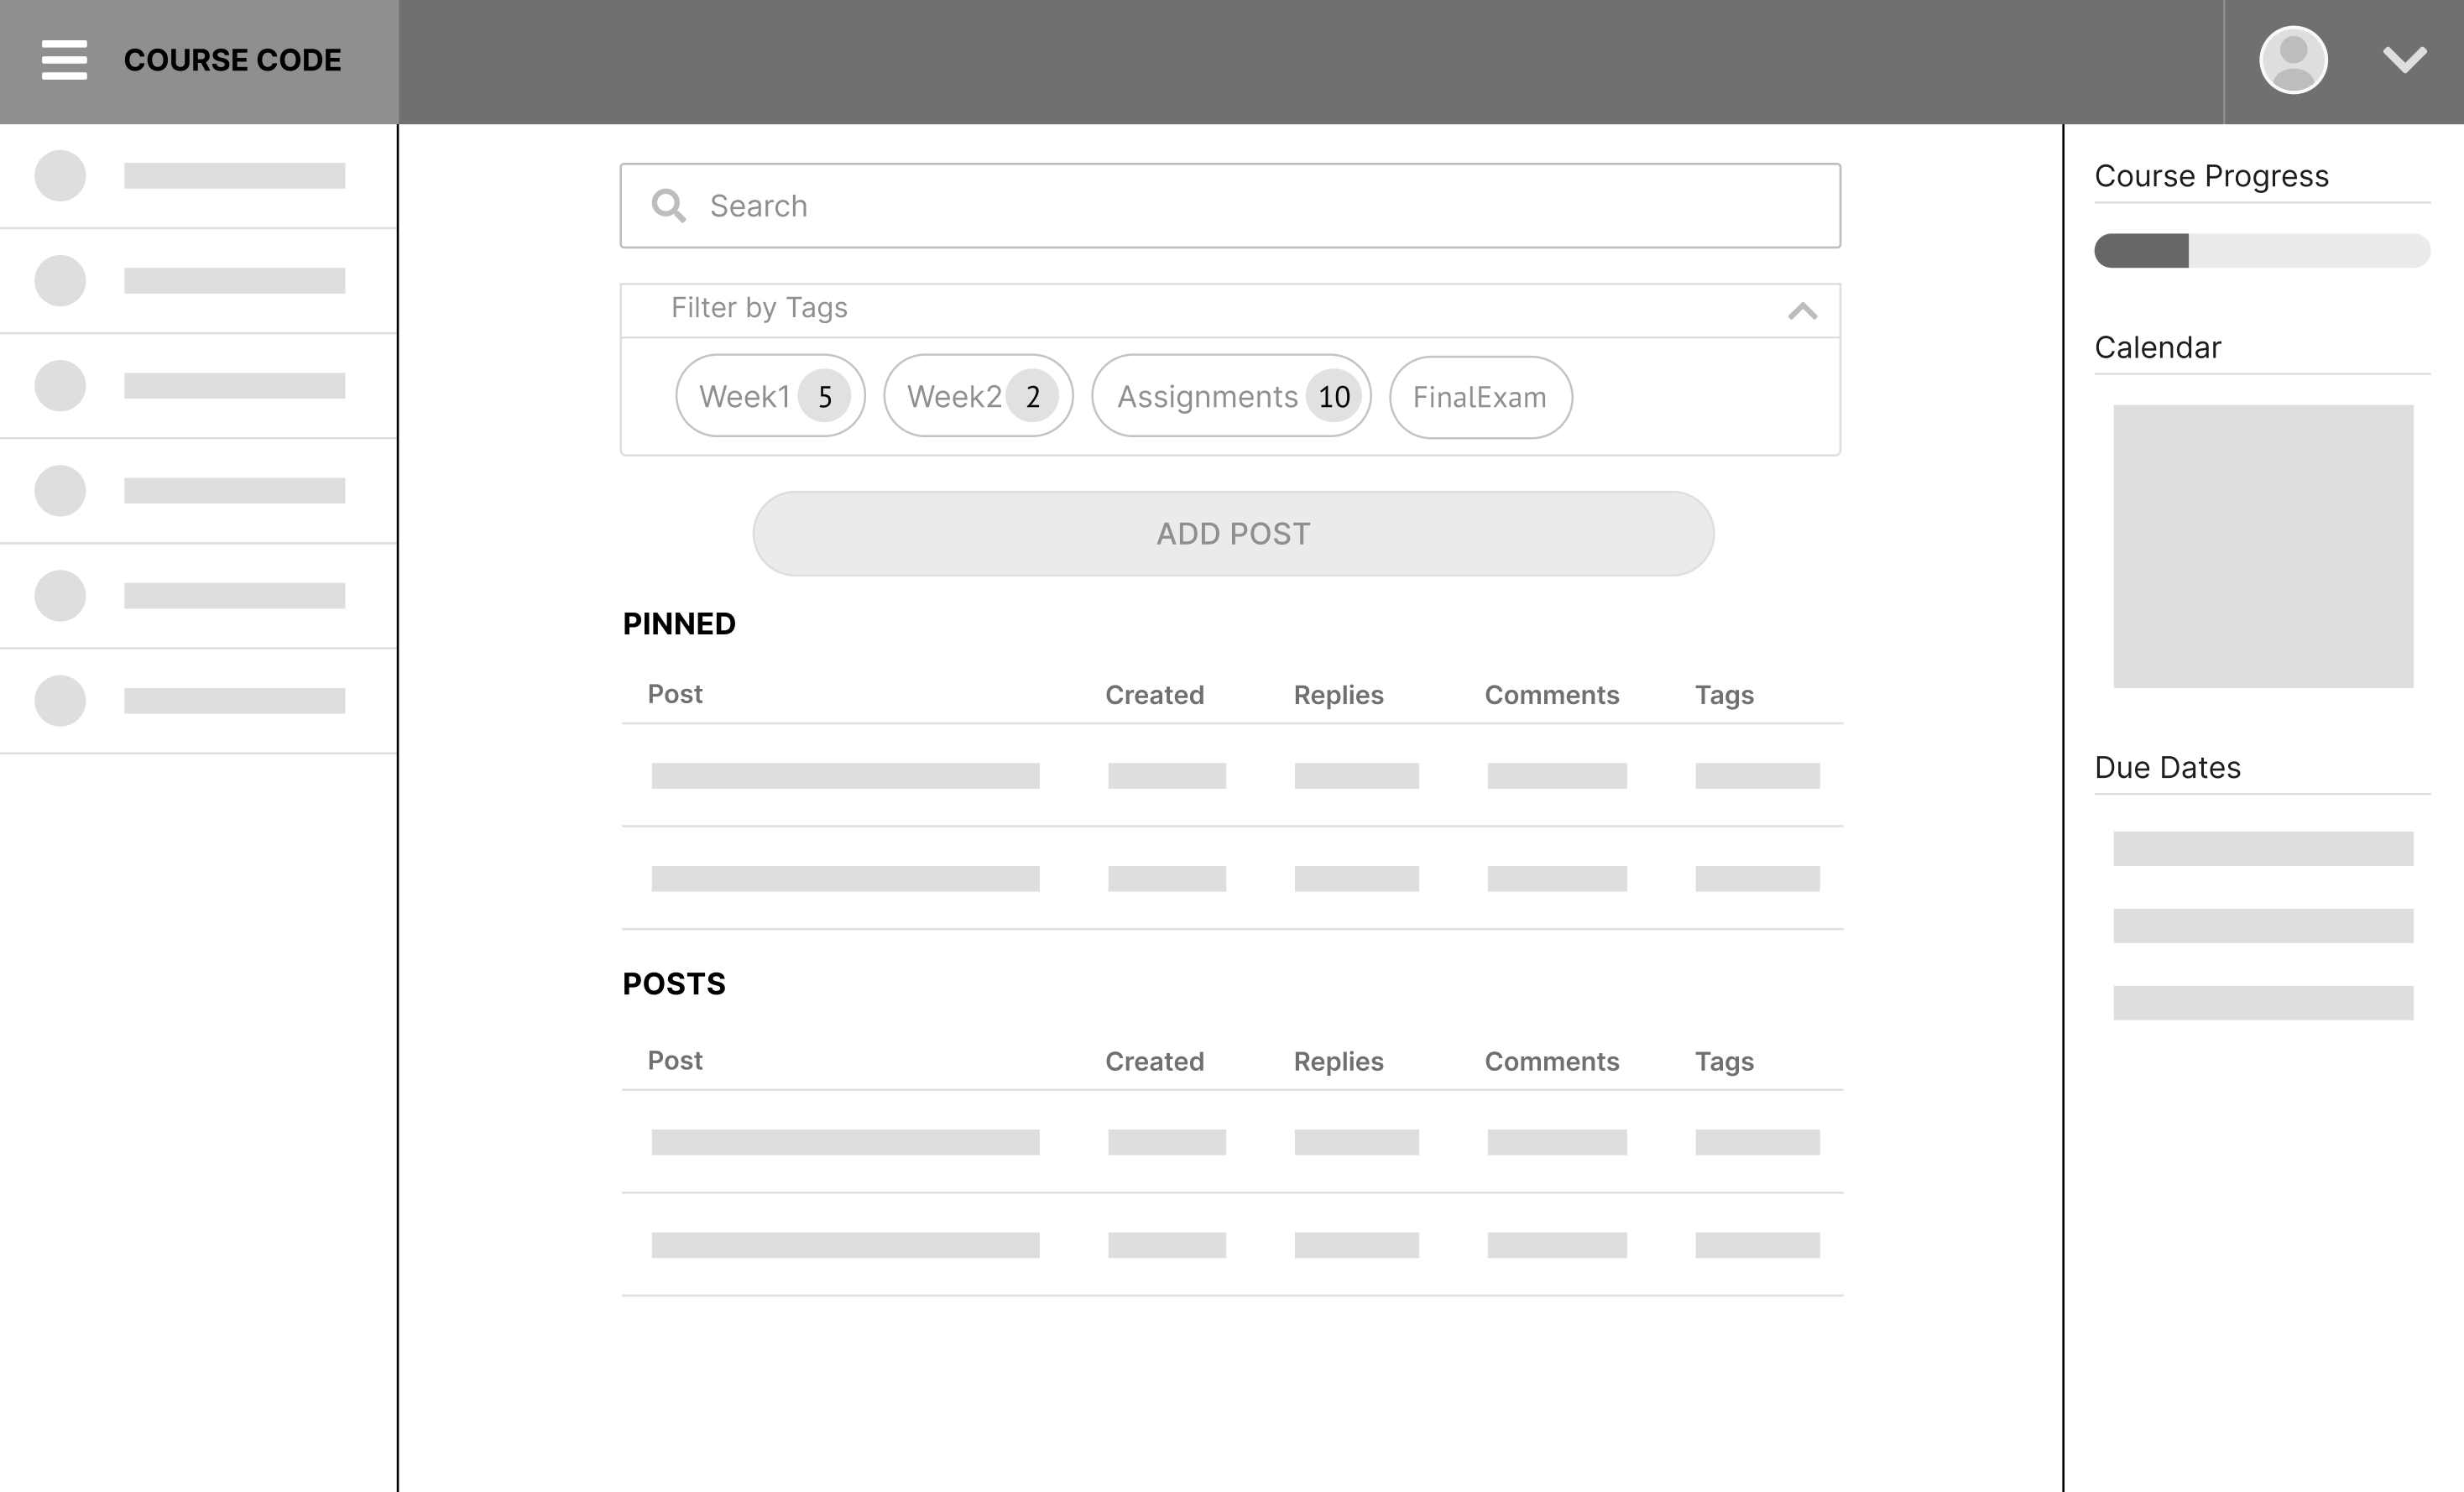
\includegraphics[scale=0.2]{forum-overview-page-student.png}
    \centering
    \caption{Forum overview page for a student}
\end{figure}

In general, the forum overview page consists of a list of posts, as well as search and filtering mechanisms.
The collapsible filter menu allows users to filter the forum post based on pre-defined tags.
Forum posts are ordered such that the list of pinned posts are at the top, followed by the remaining posts in chronological order.
Each row in the table includes the post title, date created, number of replies, number of comments and the associated tags.

\begin{figure}[h!]
    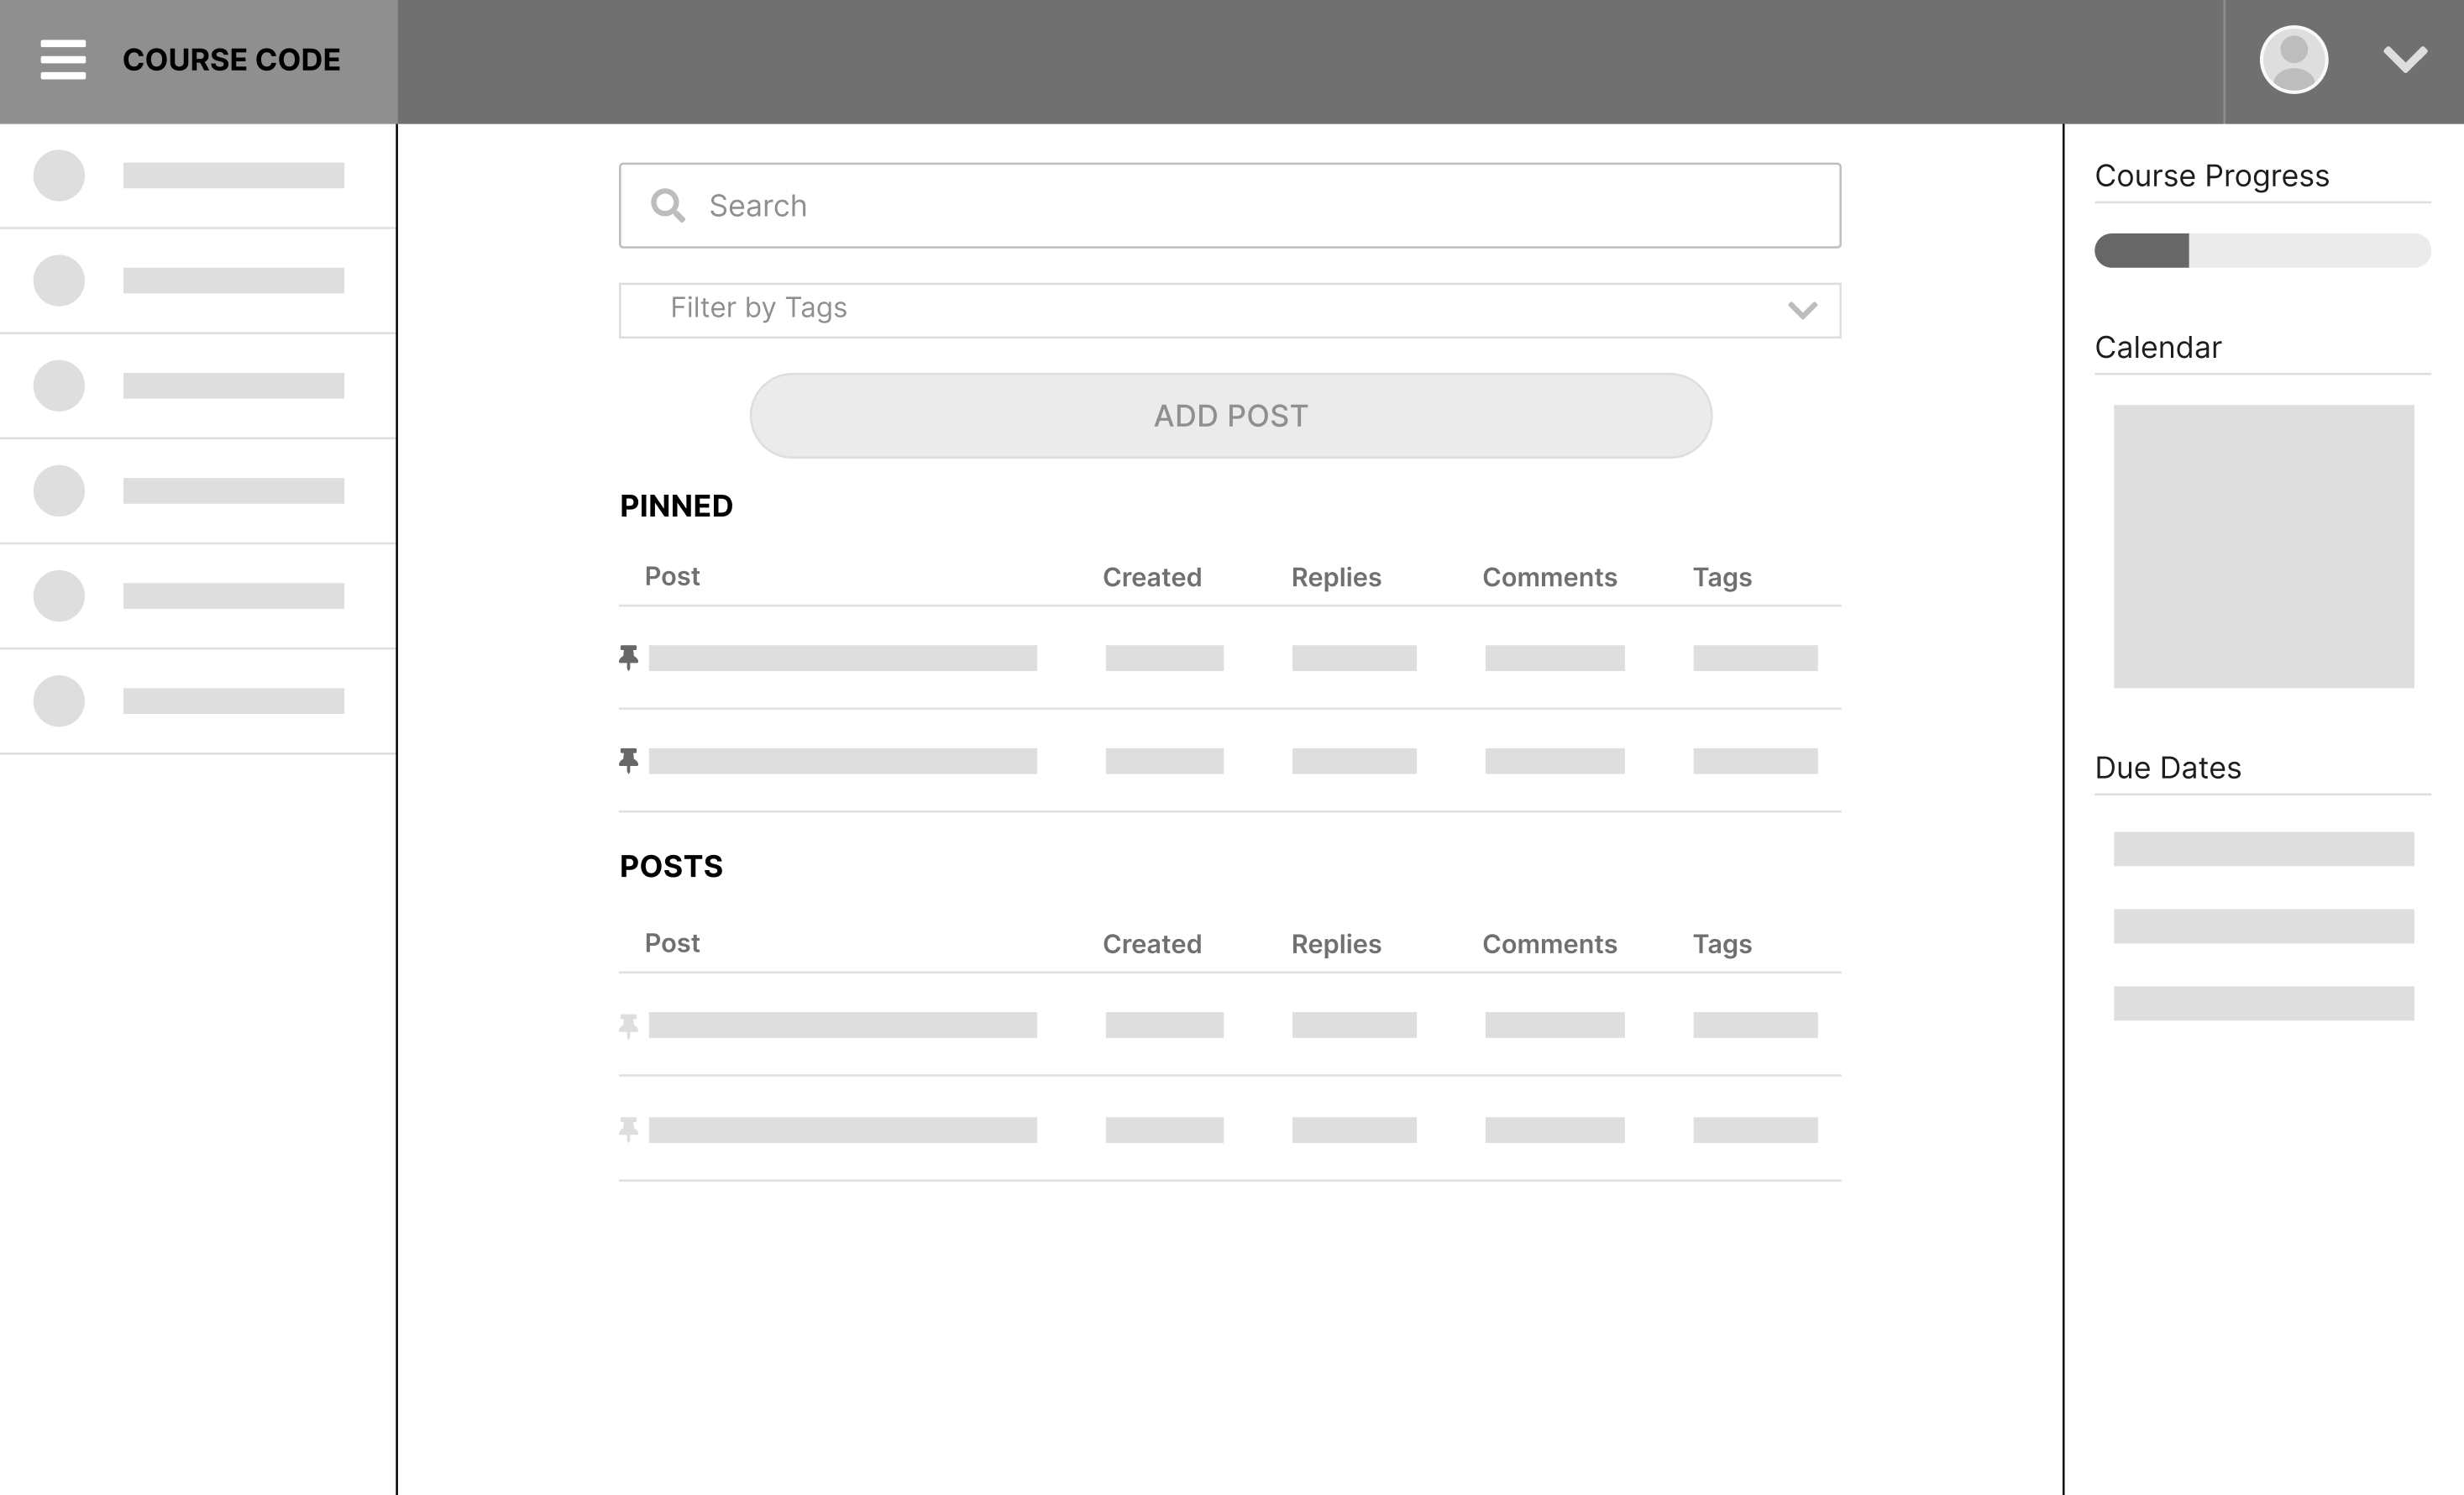
\includegraphics[scale=0.2]{forum-overview-page-admin.png}
    \centering
    \caption{Forum overview page for an admin}
\end{figure}

Admins have an additional button that allows them to pin and unpin posts.

\subsubsection{Post Page}

\begin{figure}[h!]
    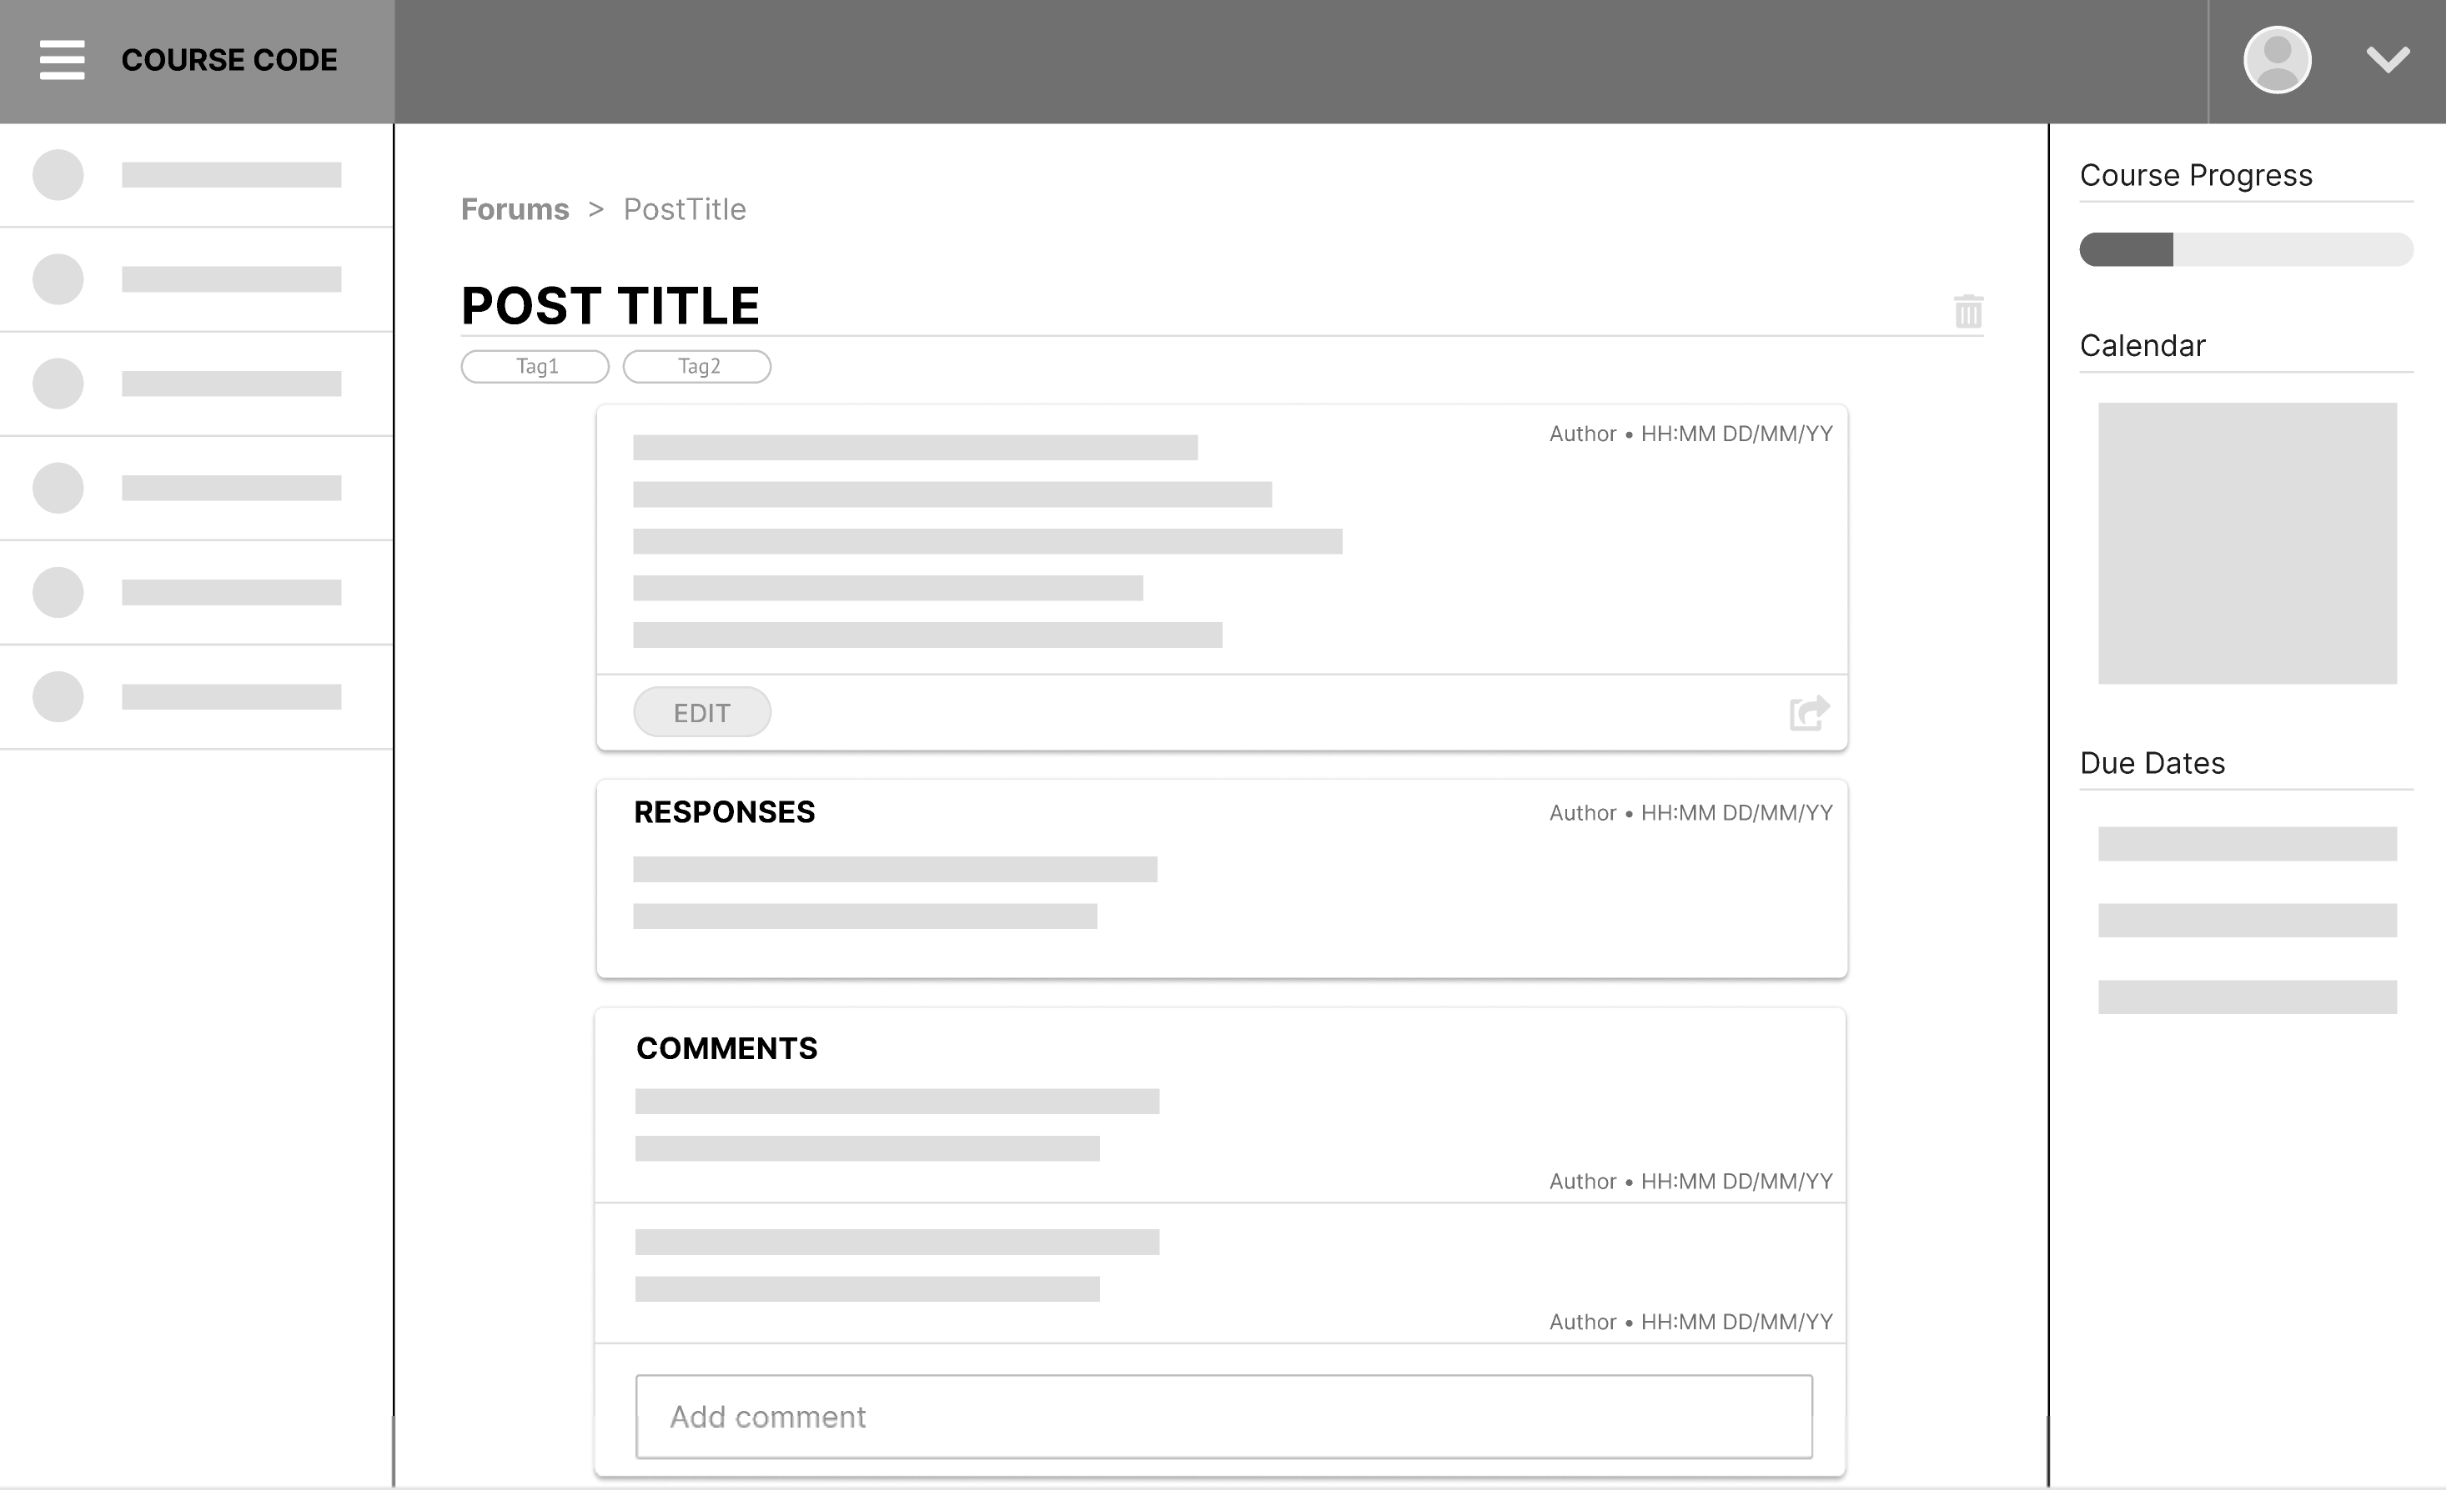
\includegraphics[scale=0.2]{forum-post-page-answered-student.png}
    \centering
    \caption{Forum post page for a student}
\end{figure}

Each forum post has its own post page which contains the post details, responses and comments.
Students are able to edit their posts from the post page if required.
They can easily view the instructor's response, if any, in the responses section.
The comments section allows the author to view and leave any additional comments.
It also gives other students a place to write a response or ask questions based on that forum post.

\begin{figure}[h!]
    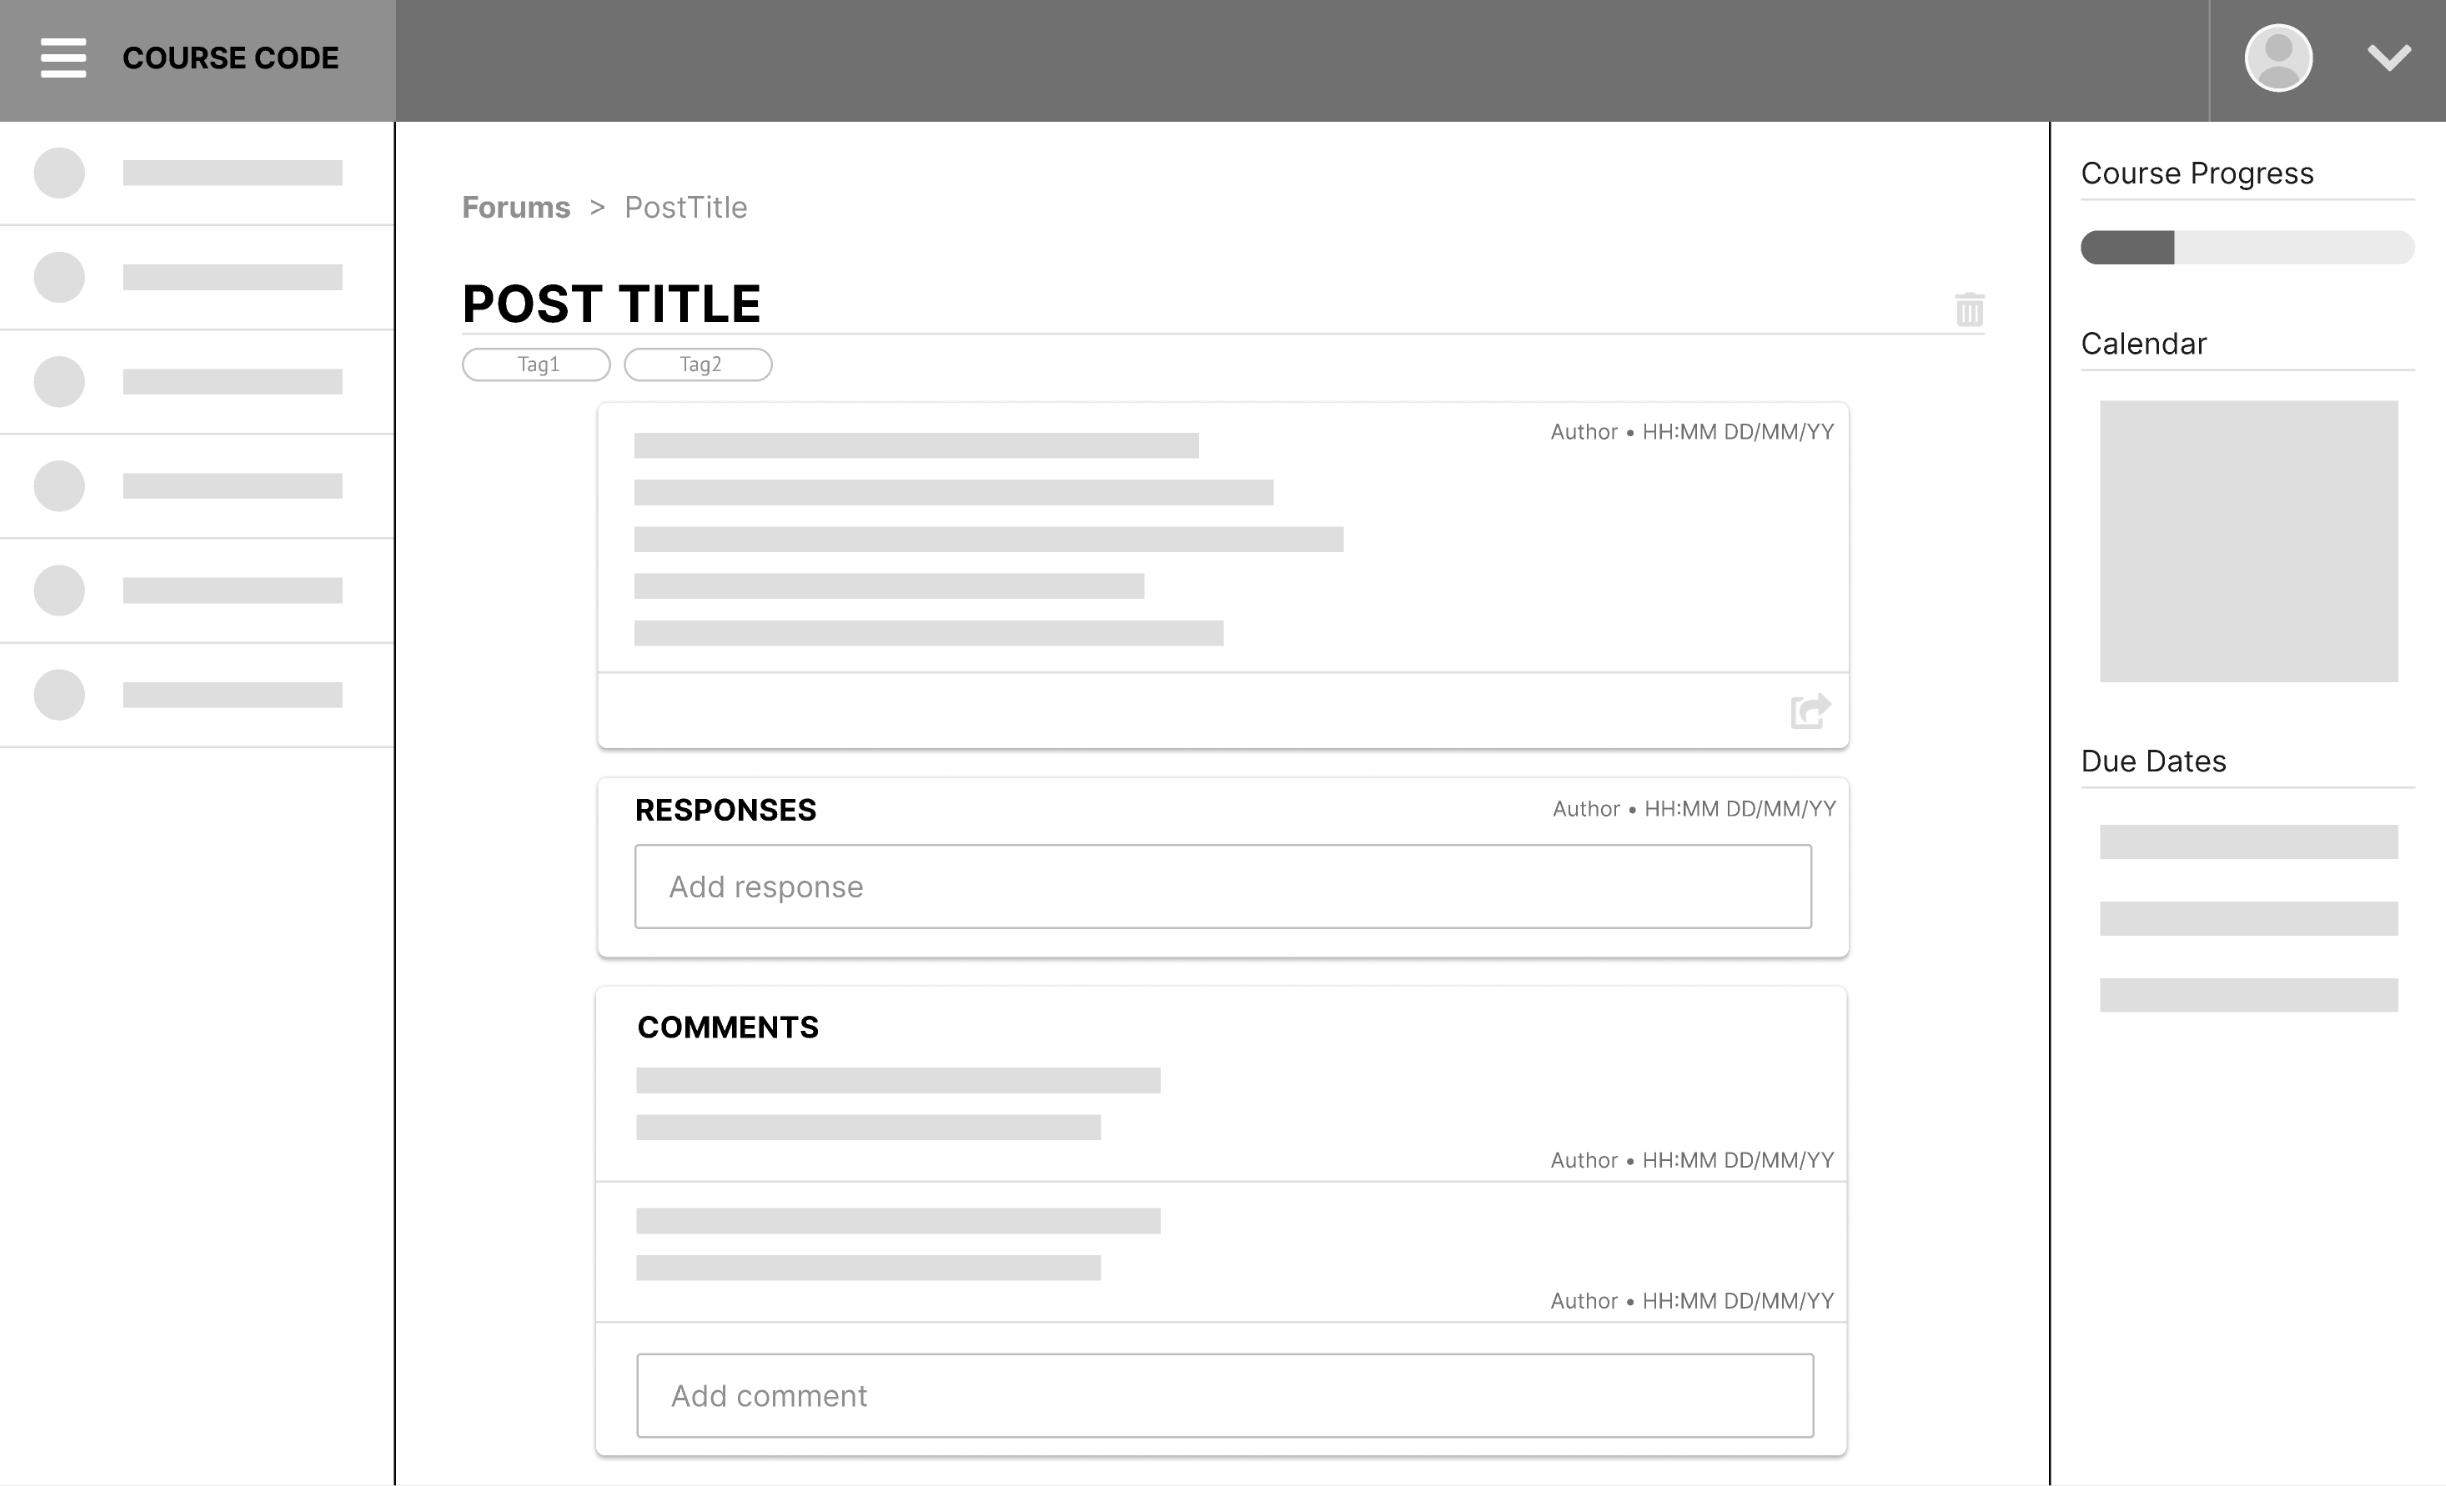
\includegraphics[scale=0.2]{forum-post-page-unanswered-admin.png}
    \centering
    \caption{Forum post page for an admin}
\end{figure}

If a forum post is unanswered, an admin is able to leave a response.
The current idea is to restrict this so that only admins can write responses to ensure that all responses are verified.
It also ensures that forum posts aren't left unanswered if a student accidentally leaves a follow-up question in the responses area, instead of the comments section.
This method of implementation may be reassessed if time allows.

\subsection{Requirements}
The following features are prioritised using the MoSCoW method which assists in identifying the order in which to implement the requirements.
It contains the following categories

\begin{itemize}
    \item \textbf{Must have} - vital features that are critical to the basic functionality of a project
    \item \textbf{Should have} - important features that aren't critical but add to the basic functionality of a project
    \item \textbf{Could have} - desired features that aren't necessary to the overall project but can provide a better user experience
    \item \textbf{Won't have} - low-priority features that likely won't be able to be completed in the given time-frame
\end{itemize}

\subsubsection{Functional Requirements}
\begin{enumerate}
    \item Users can view a list of forum posts (Must have)
    \item Users can make posts to the forum (Must have)
    \item Users can reply to forum posts (Must have)
    \item Users can embed images and links in their posts (Should have)
    \item Users can share forum posts (Should have)
    \item Users can categorise forum posts (Should have)
    \item Users can search forum posts (Should have)
    \item Users can clearly see which posts have been read and actioned (Could have)
    \item Admins can pin important forum posts (Should have)
    \item Admins can link/embed materials to forum posts (Could have)
    \item Admins can curate forum questions into collections (Won't have)
\end{enumerate}

\subsection{Backend Assumptions}
Since the backend for the Meta LMS is being built out independently to the individual features, the following contains a description of the ideal backend design for the forum component.

\subsubsection{Database}
The main database table required for this component is one to store all the forum posts.
This would include all the post details including author, title, description, date created and tags.
It would also need to have a way to keep track of the replies and comments left on the forum post.
This could either be done by having separate tables for replies and comments, or by storing a list of replies and comments within each forum post entry.
For each of the forum posts, the author would need to be linked to a user in the user table of the database.

\subsubsection{API}
In terms of the backend API, the following functionality would be required in order to store, retrieve and update the appropriate data from the database.

\begin{enumerate}
    \item Retrieve a list of all forum posts
    \item Retrieve a list of the pinned posts
    \item Retrieve a list of posts related to search term
    \item Retrieve a list of posts related to filter
    \item Retrieve individual post details for post page (including comments and responses)
    \item Store new post details
    \item Store post responses
    \item Store post comments
    \item Update post details when author edits post
    \item Update response when author edits response
    \item Update pinned post list when admin pins/unpins posts
\end{enumerate}

\subsection{Project Timeline}
Below is a rough guideline of some milestones that should be met throughout the year in order to complete this feature on time.

\subsubsection{Thesis A}
The focus of Thesis A, Term 1 2021, is solely based around researching current learning management systems to get a good understanding of the desired features required for a meta LMS.
It also includes more in-depth research of forums and planning out what this forum component should consist of.

\begin{figure}[h!]
    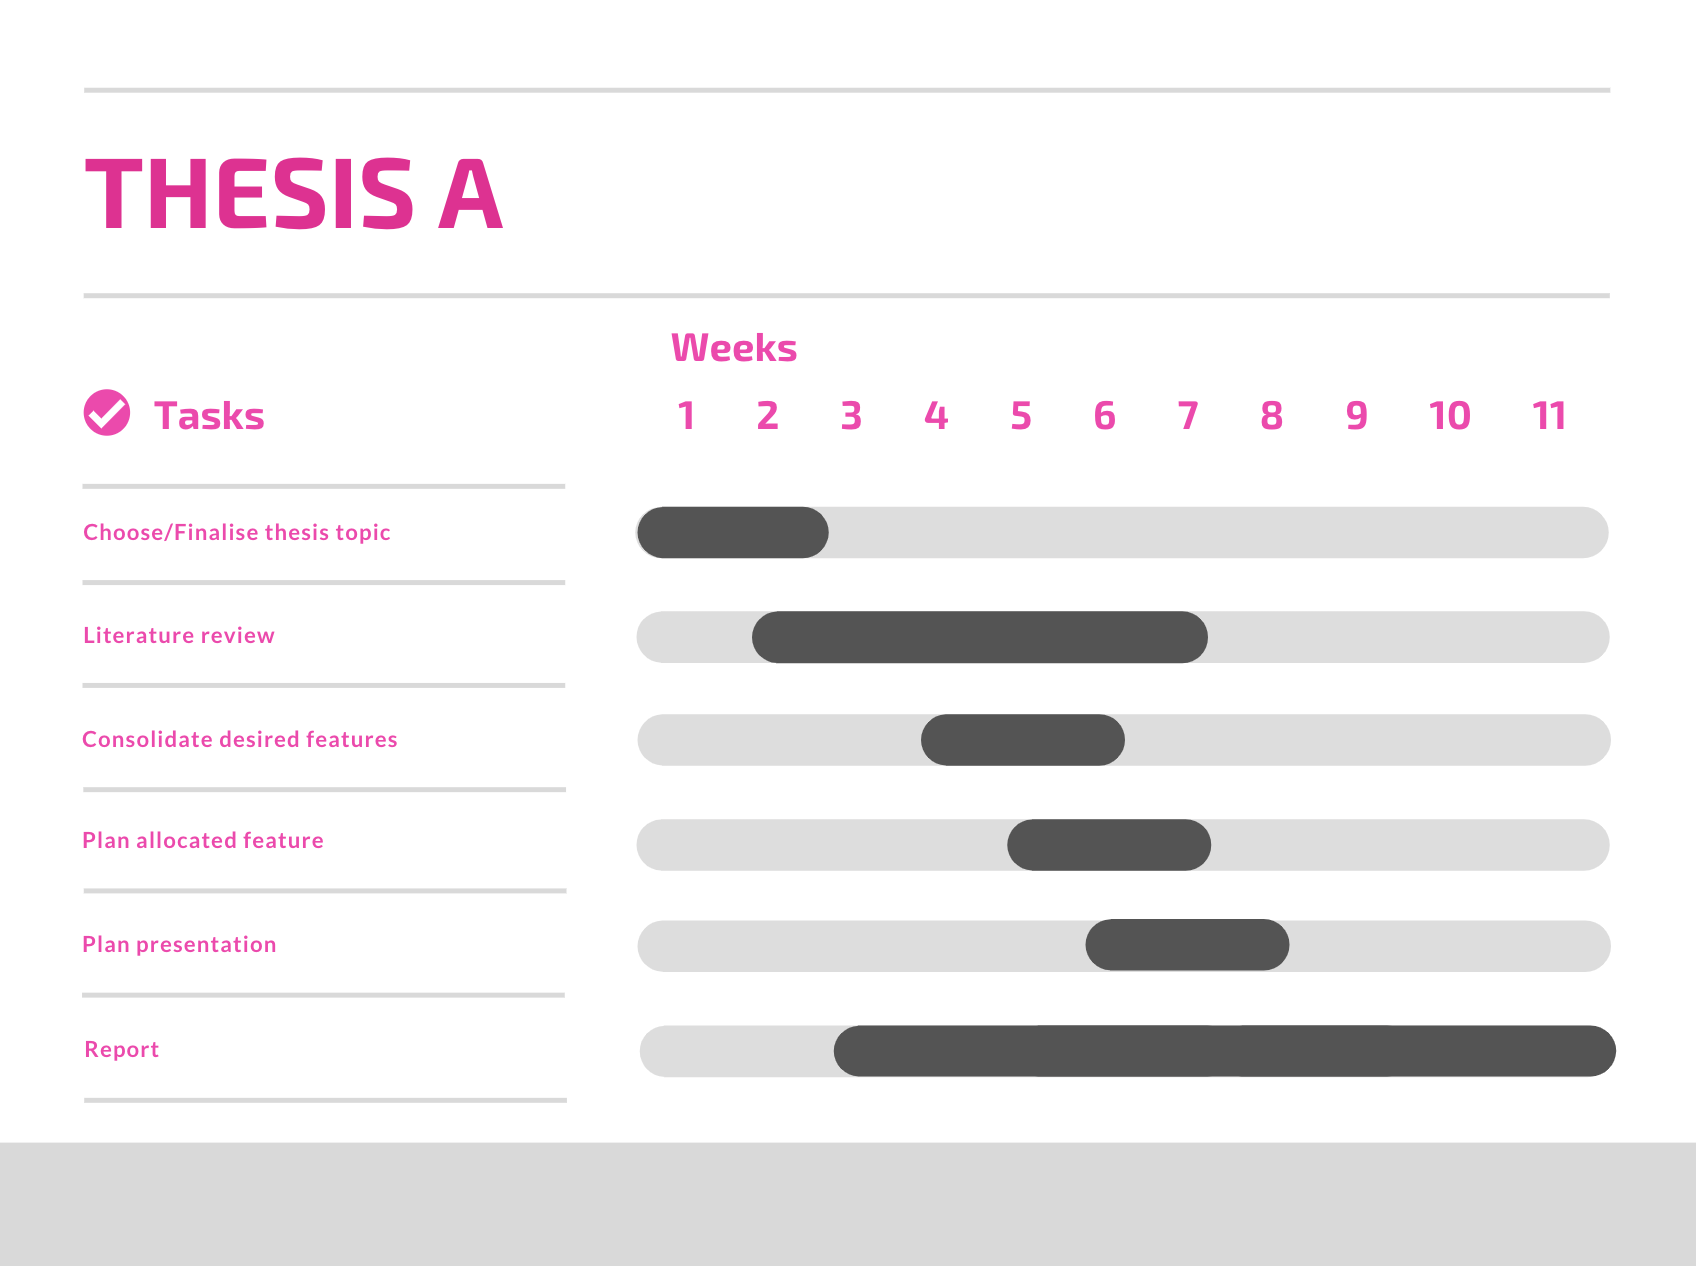
\includegraphics[scale=0.4]{forum-thesis-a.png}
    \centering
    \caption{Thesis A Timeline}
\end{figure}

\newpage

\subsubsection{Thesis B}
Thesis B, Term 2 2021, will hopefully consist of most of the implementation work for forums.
It will start with some market research to get a good understanding of the wants and needs to students and educators.
Analysis of these results will help to finalise the features and designs of the forum component.

Once the frontend and backend designs have been finalised, the forum overview page and post page will be implemented.
This includes viewing posts, making posts and replying to posts.

The next focus is the searching and filtering functionalities.
This includes searching the forum and filtering based on pre-defined tags.

Finally, in Thesis B, the ability to pin and share posts will be added.
This should conclude the implementation of all the main features of the forum component.

\begin{figure}[h!]
    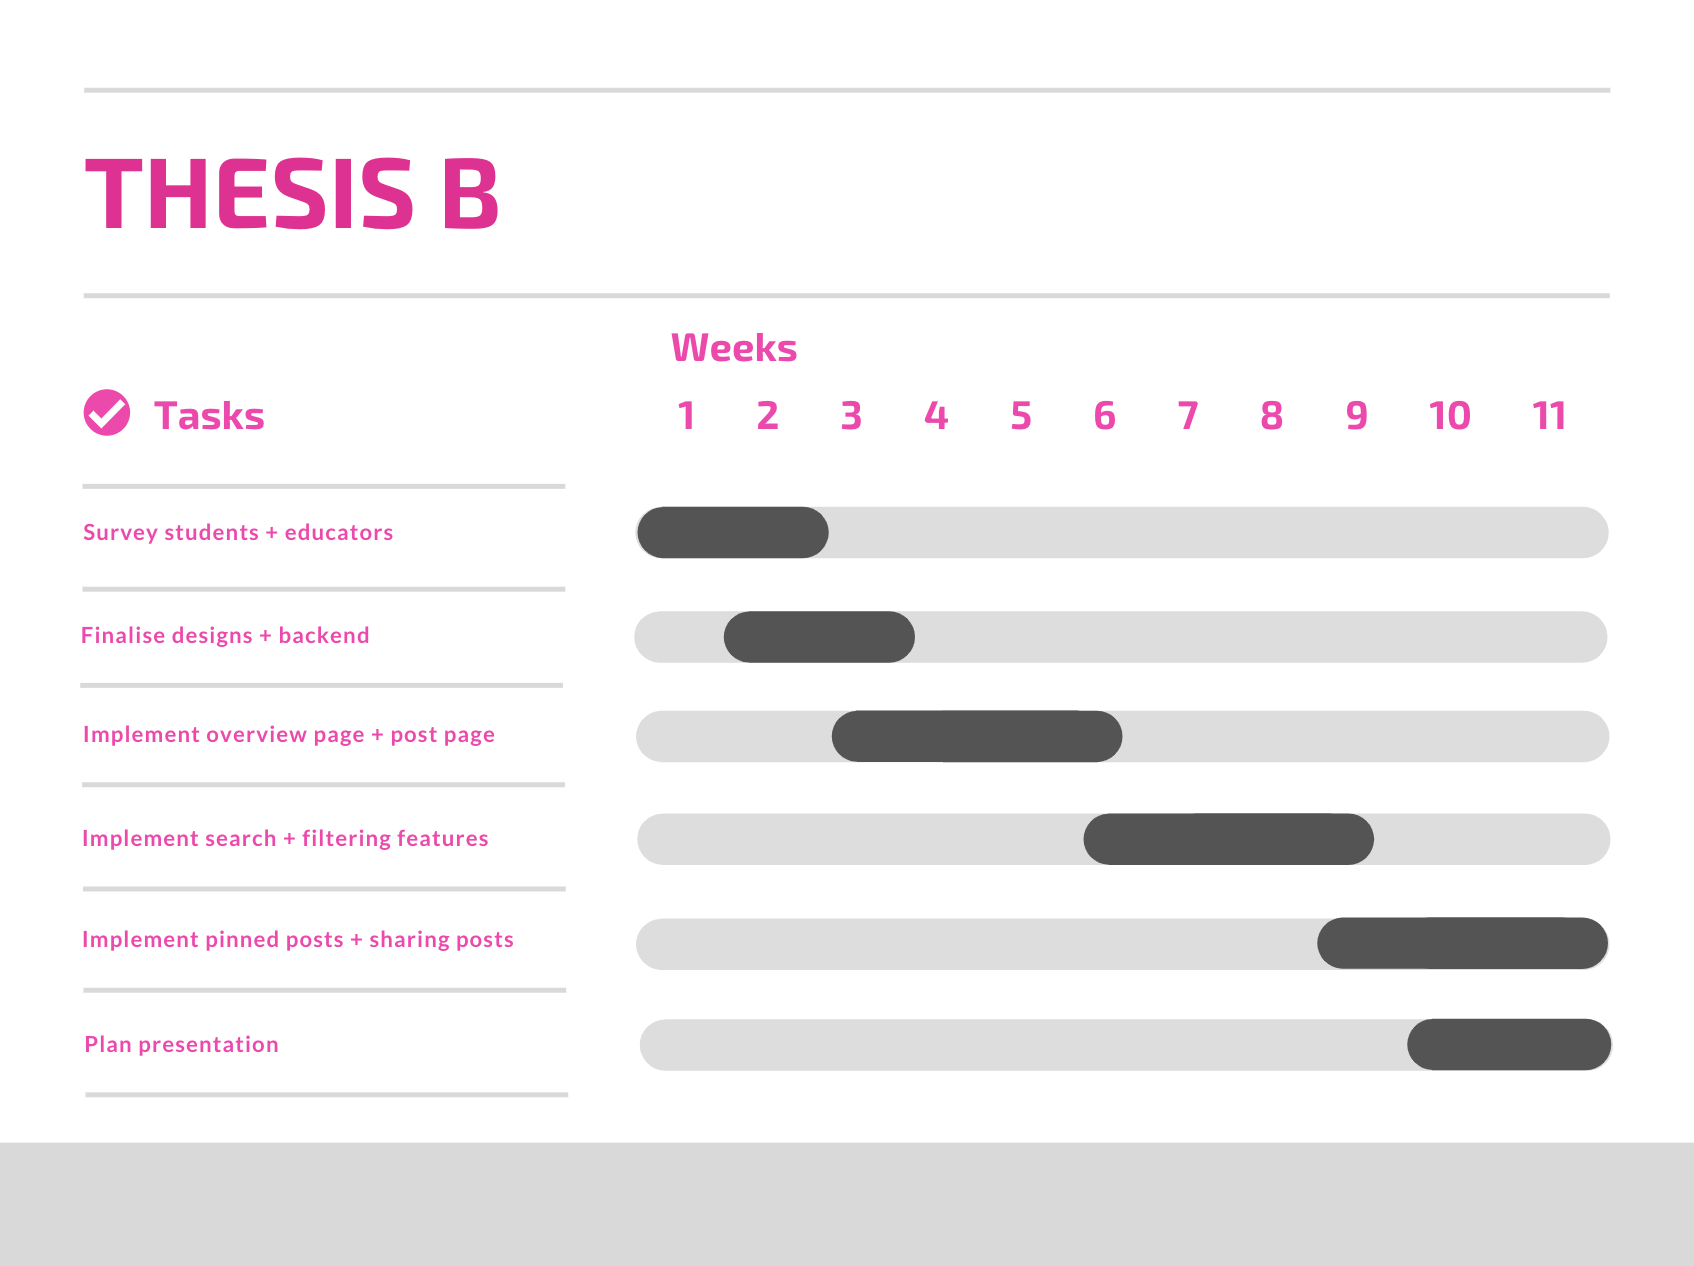
\includegraphics[scale=0.4]{forum-thesis-b.png}
    \centering
    \caption{Thesis B Timeline}
\end{figure}

\subsubsection{Thesis C}
Thesis C, Term 3 2021, is mainly centred around finalising the implementation and evaluating the solution.
The first few weeks will consist of completing any unfinished features, cleaning up the UI and debugging any problems.
If there is time, extra features could be implemented.
Time will also be allocated to integrating the forum with the rest of the LMS.

The middle weeks of the term will focus on analysis and usability testing.
This will help see if the users' needs have been met by the implemented solution.

The final few weeks will consist of any final improvements and testing.
The results from the analysis will help to fix any problems with the forum component.

\begin{figure}[h!]
    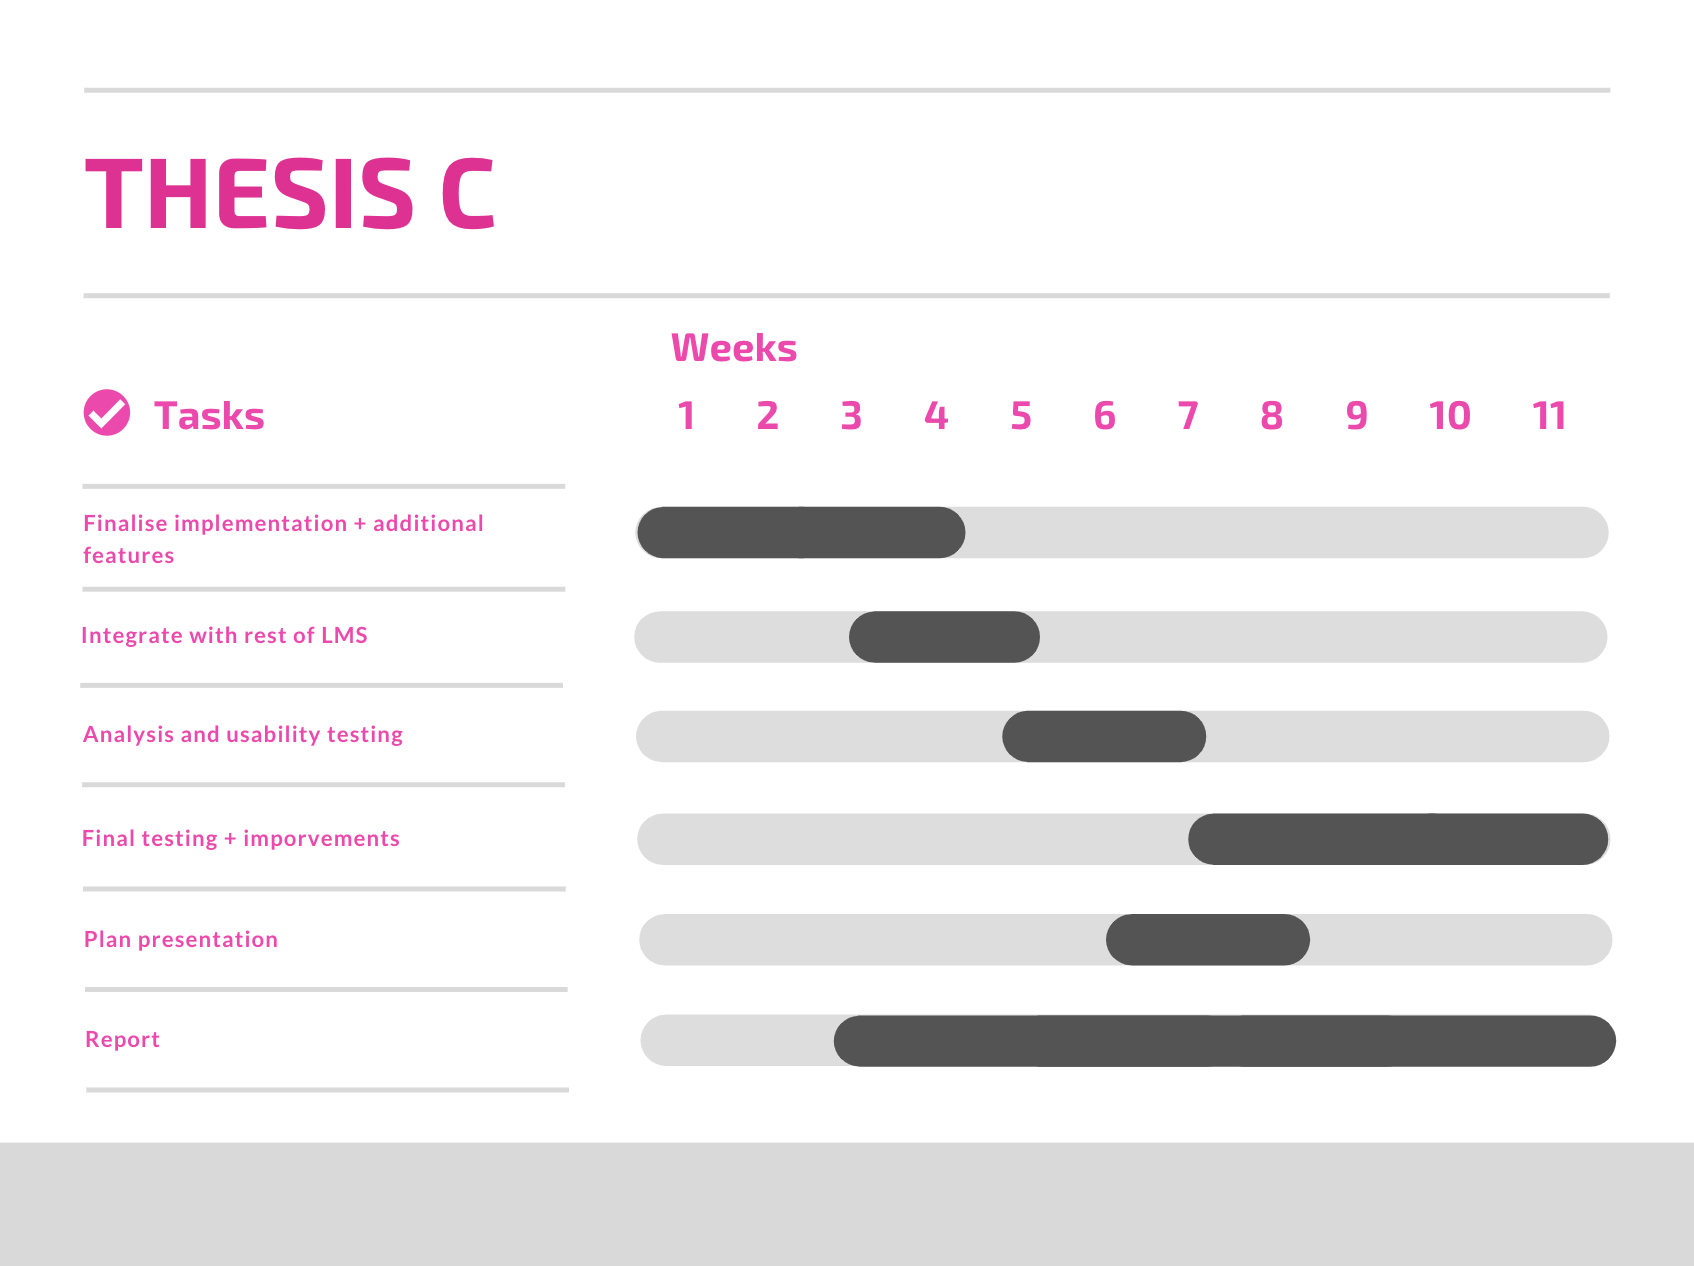
\includegraphics[scale=0.4]{forum-thesis-c.png}
    \centering
    \caption{Thesis C Timeline}
\end{figure}